\documentclass[letter,12pt]{article}
\usepackage[left=2.54cm, right=2.54cm, top=2.54cm, bottom=2.54cm]{geometry} % Márgenes APA
\usepackage{setspace} % Interlineado
\setlength{\parindent}{1.27cm} % Sangría estándar APA
\setlength{\parskip}{0pt}     % Sin espacio entre párrafos
\usepackage{graphicx} % Para insertar imágenes
\usepackage{float} % Para posicionar imágenes y tablas
\usepackage{caption} % Para modificar captions de tablas e imágenes
\usepackage{csquotes} % Para mejor manejo de citas
\usepackage{amsmath} % Para ecuaciones matemáticas
\usepackage{svg}
\usepackage{indentfirst}

%==========REFERENCIAS=============
\usepackage[backend=bibtex,style=ieee,biblabel=dot,language=spanish]{biblatex}
\addbibresource{referencias.bib}

\usepackage[
    xetex,
    pdftitle={Tarea \# 1 - FFT y Sistemas de Modulación}, % Título del PDF
    pdfauthor={Barquero, J., Feng, J., Montero, A.},   % Autor del PDF
    pdfsubject={CE1110 - Análisis de Señales Mixtas}, % Tema del PDF
    pdfkeywords={}, % Palabras clave del PDF
    pdfproducer={LaTeX with hyperref package},
    pdfcreator={pdfLatex}
]{hyperref}

\hypersetup{
    colorlinks=true,        % Colorea los enlaces en lugar de usar cajas alrededor de ellos
    linkcolor = black,
    urlcolor  = blue,
    citecolor = black,
    anchorcolor = blue         % Color de los enlaces externos
}

\begin{document}
% ====== Portada ======
\begin{titlepage}
    \centering
    {\LARGE \textbf{Tarea \# 1} \par}
    {\LARGE FFT y Sistemas de Modulación \par}
    \vspace{1.5cm}
    {\large José Bernardo Barquero Bonilla \\ 2023150476 \par}
    {\large Jimmy Feng Feng \\ 2023060347 \par}
    {\large Alexander Montero Vargas \\ 2023166058 \par}
    \vspace{1.5cm}
    {\Large Instituto Tecnológico de Costa Rica \par}
    {\large Escuela de Ingeniería en Computadores \par}
    {\large Curso: CE1110 - Análisis de Señales Mixtas \par}
    \vspace{1.5cm}
    {\large Profesor: Luis Alberto Chavarría Zamora \par}
    \vfill
    {\large 15 de Octubre de 2025 \par}
\end{titlepage}

% ====== Desarrollo ======
\section{DFT/FFT y serie de Fourier}

La Transformada Discreta de Fourier (DFT) es la definición matemática que proyecta una secuencia finita \(x[n]\) de longitud \(N\) sobre exponenciales complejas y entrega \(N\) muestras espectrales \(X[k]\) igualmente espaciadas en frecuencia \cite{OppenheimSchaferDTSP3e,VetterliKovacevicGoyalFSP2014}. La DFT se calcula como
\[
X[k]=\sum_{n=0}^{N-1} x[n]\,e^{-j2\pi kn/N},\quad k=0,\dots,N-1,
\]
y la inversa como
\[
x[n]=\frac{1}{N}\sum_{k=0}^{N-1} X[k]\,e^{+j2\pi kn/N},\quad n=0,\dots,N-1.
\]
Estas expresiones fijan la convención de normalización usada a lo largo del documento \cite{OppenheimSchaferDTSP3e}.

La Transformada Rápida de Fourier (FFT) no es una transformada distinta, sino un algoritmo que evalúa la DFT con complejidad \(O(N\log N)\), en contraste con los \(O(N^2)\) de la evaluación directa \cite{CooleyTukey1965}. En la práctica, “hacer una FFT” significa calcular la DFT de forma eficiente; la distinción es: \emph{qué} se calcula (DFT) versus \emph{cómo} se calcula (FFT) \cite{OppenheimSchaferDTSP3e,NumPyFFT2024}.

Para una señal discreta \(x[n]\), la transformada \(X(e^{j\omega})\) (DTFT) es continua en \(\omega\) y periódica con período \(2\pi\) \cite{OppenheimSchaferDTSP3e,NISTDLMF_Fourier}:
\[
X(e^{j\omega})=\sum_{n=-\infty}^{\infty} x[n]\,e^{-j\omega n},\qquad
X(e^{j(\omega+2\pi)})=X(e^{j\omega}).
\]
La DFT puede interpretarse como un \emph{muestreo} de esta DTFT en \(N\) frecuencias uniformemente espaciadas \( \omega_k=2\pi k/N \), o en Hz \( f_k=\tfrac{k}{N}f_s \), con resolución \(\Delta f=\tfrac{f_s}{N}\) \cite{OppenheimSchaferDTSP3e,VetterliKovacevicGoyalFSP2014,SciPyFFT2024}. Aumentar \(N\) mejora la resolución; el \emph{zero-padding} densifica la grilla de lectura sin aumentar la resolución física \cite{SciPyFFT2024,NumPyFFT2024}.

La relación con la serie de Fourier surge de la periodicidad. La serie de Fourier representa una señal periódica continua \(x(t)\) como suma de armónicos discretos \(k f_0\) con coeficientes \(c_k\) \cite{OsgoodFTAMS2019,NISTDLMF_Fourier}:
\[
x(t)=\sum_{k=-\infty}^{\infty} c_k\,e^{j2\pi k f_0 t},\qquad
c_k=\frac{1}{T_0}\int_{0}^{T_0} x(t)\,e^{-j2\pi k f_0 t}\,dt.
\]
Análogamente, al tomar un bloque de \(N\) muestras y asumir su repetición periódica en tiempo discreto, la DFT entrega los coeficientes de la serie de Fourier de esa señal periódica discreta: tiempo (discreto) periódico \(\Rightarrow\) espectro (discreto) en \(N\) líneas \cite{OppenheimSchaferDTSP3e,VetterliKovacevicGoyalFSP2014}.

Finalmente, respecto al “muestreo del entorno continuo”, muestrear \(x(t)\) cada \(T_s\) genera \(x[n]=x(nT_s)\) y replica el espectro continuo \(X_c(f)\) cada \(f_s=1/T_s\); si \(f_s<2f_{\max}\) ocurre aliasing \cite{OppenheimSchaferDTSP3e,OsgoodFTAMS2019}. Sobre esta señal ya discreta, la DFT toma muestras de la DTFT en los bins \(f_k\), cerrando la cadena conceptual: muestreo temporal \(\Rightarrow\) réplicas en frecuencia; ventana temporal \(\Rightarrow\) suavizado por convolución; DFT/FFT \(\Rightarrow\) muestreo uniforme del espectro discreto-periódico \cite{OppenheimSchaferDTSP3e,SciPyFFT2024}.



% =========================
\section{Experimento 1: FFT sobre audio libre}

\subsection{Datos y preparación}

Se utilizó una pista de audio libre en formato WAV con frecuencia de muestreo \(f_s=44{,}100\) Hz. Del audio completo se seleccionó el tramo de \(t\in[8,\,20.7]\) s, de duración efectiva \(T\approx 12.696\) s, convertido a mono por promediado de canales y normalizado a \([-1,1]\) antes del análisis. Este preprocesamiento evita sesgos de escala y asegura que la potencia esté acotada para una interpretación coherente de magnitud y fase en la FFT \cite{OppenheimSchaferDTSP3e}.  

La lectura del WAV se realizó con una rutina estándar que ignora metadatos no audio (advertencia \emph{Chunk (non-data) not understood}), lo cual no afecta las muestras útiles. El objetivo del experimento es estimar el espectro de magnitud \(|X(f)|\) y la fase \(\angle X(f)\) de una señal compuesta por dos senoidales muy cercanas en frecuencia, un caso clásico para estudiar resolución en frecuencia, batido temporal y fuga espectral \cite{oppenheim2010}.

\subsubsection{Configuración de análisis}

Se empleó una ventana de Hann sobre el segmento seleccionado. La elección de Hann ofrece un buen compromiso entre atenuación de lóbulos laterales y ensanchamiento del lóbulo principal, lo que mitiga la fuga espectral sin degradar en exceso la separabilidad de líneas cercanas \cite{Harris1978Windows}.  

Con el tramo elegido se obtuvo un tamaño base para la FFT de \(N_{\text{base}}=912{,}712\) muestras, lo que implica una resolución física en frecuencia
\[
\Delta f \;=\; \frac{f_s}{N_{\text{base}}} \;\approx\; \frac{44{,}100}{912{,}712}\;\approx\;0.0483\ \text{Hz}.
\]
Para las figuras presentadas no se aplicó \emph{zero padding} adicional (\(\text{zp}\times1\)), de modo que la rejilla de frecuencias coincide con \(\Delta f\) física. Se recuerda que el \emph{zero padding} sólo densifica la rejilla de muestreo en frecuencia pero no mejora la resolución física, que sigue estando gobernada por \(N_{\text{base}}\) \cite{OppenheimSchaferDTSP3e}.  

En una pareja de tonos separados por un centésimo de semitono musical, la separación esperada es
\[
\Delta f_{\text{cent}} \;\approx\; f_0\big(2^{1/1200}-1\big),
\]
que para \(f_0\approx 261\) Hz da \(\Delta f_{\text{cent}}\approx 0.15\) Hz. El batido en tiempo tiene periodo aproximado \(T_{\text{beat}}\approx 1/\Delta f\), por lo que se espera observar una envolvente lenta en el dominio temporal \cite{CooleyTukey1965}.

\subsection{Resultados espectrales}

La Figura~\ref{fig:exp1-waveform} muestra la forma de onda del segmento analizado. Se aprecia una envolvente lenta de batido, consistente con la superposición de dos senoidales muy próximas y con el valor esperado de \(T_{\text{beat}}\) a partir de la separación en frecuencia \(\Delta f\) \cite{OppenheimSchaferDTSP3e}.  

% ======= FIGURAS (manteniendo rutas y nombres provistos) =======

% ===== Figura 1 =====
\begin{figure}[H]
  \centering
  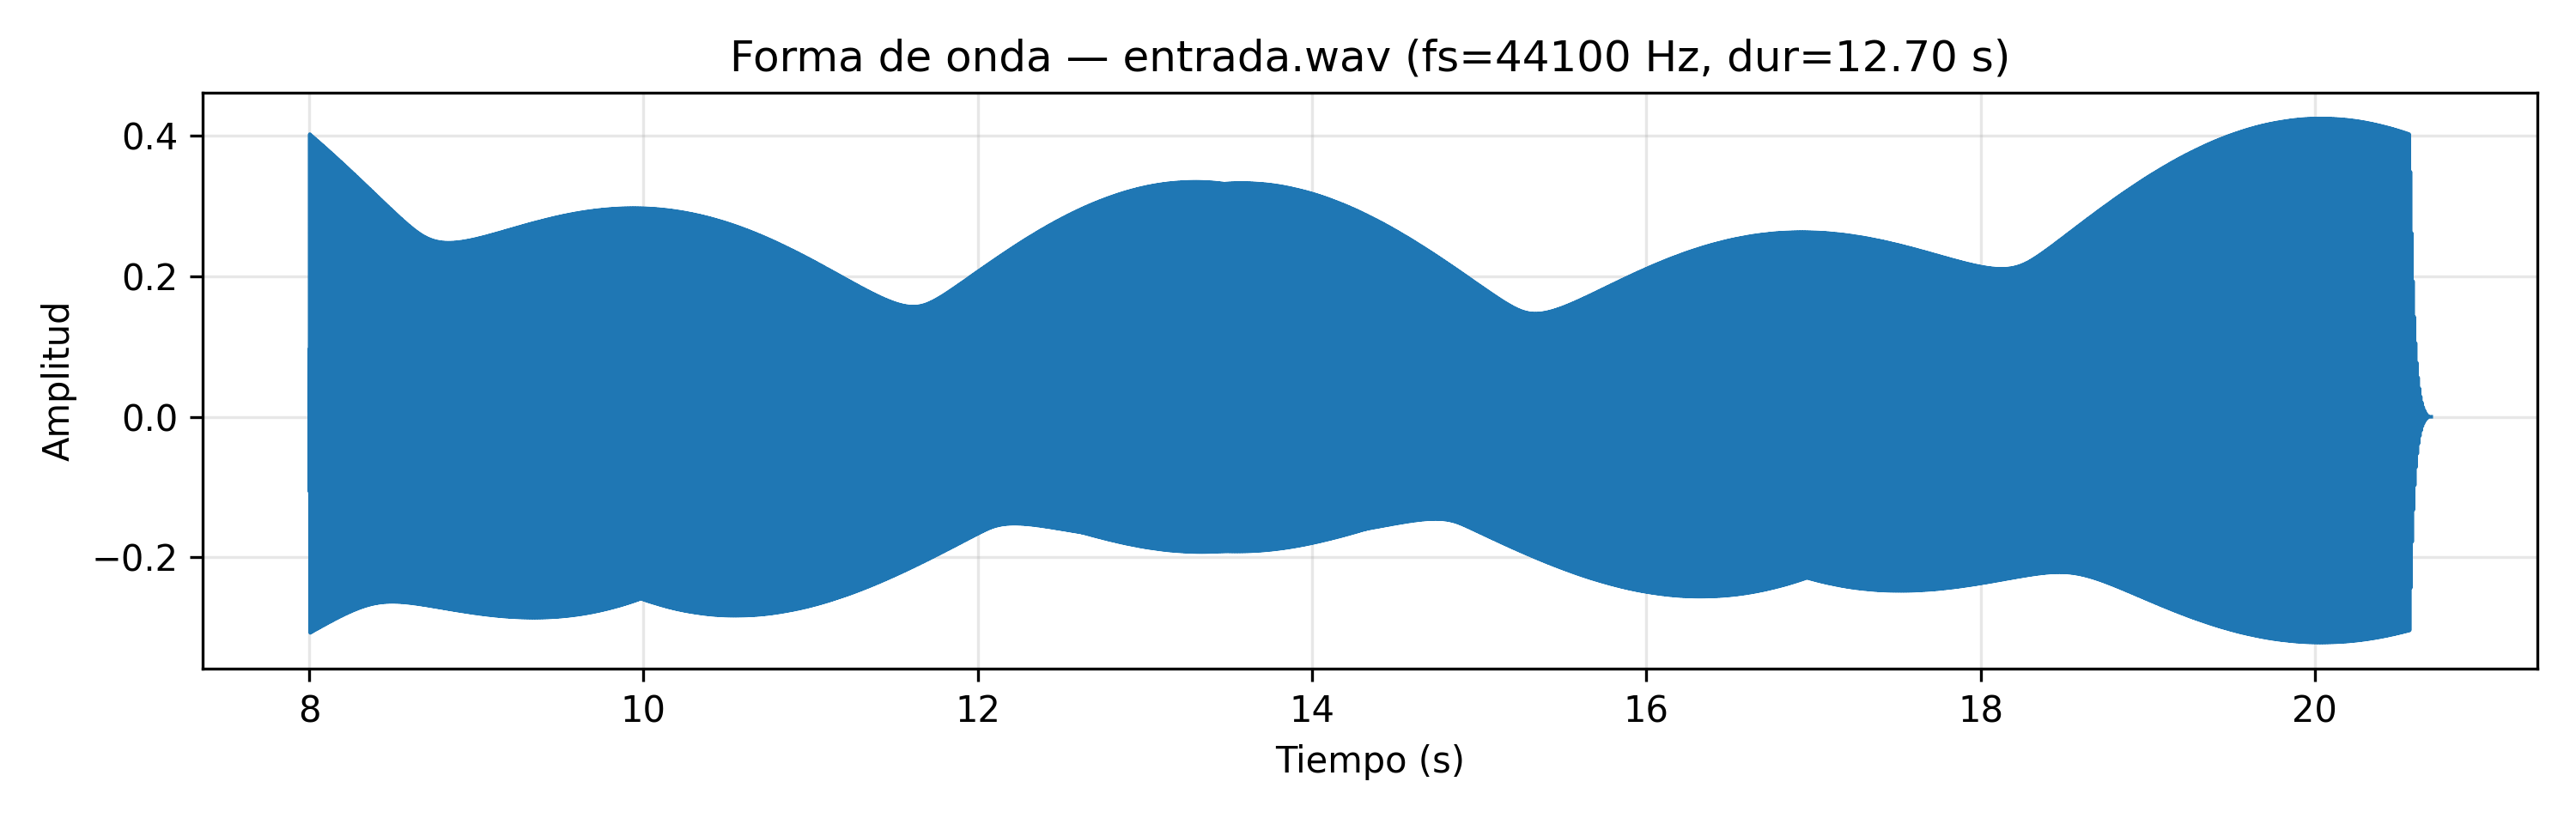
\includegraphics[width=0.98\linewidth]{Media/Figura1.png}
  \caption{Forma de onda del segmento analizado con \(f_s=44.1\) kHz. Se observa una envolvente de batido producida por dos componentes senoidales muy cercanas en frecuencia. El fenómeno temporal es consistente con la separación en frecuencia que se confirma en el dominio espectral.}
  \label{fig:exp1-waveform}
\end{figure}

En la Figura~\ref{fig:exp1-mag-full} se observa un pico dominante alrededor de \(261\) Hz y componentes en \(\sim131\) Hz y \(\sim524\) Hz, consistentes con relación de octavas del material analizado. La energía fuera de esas vecindades cae de forma marcada gracias al uso de ventana de Hann, que atenúa la fuga espectral al reducir los lóbulos laterales respecto de una ventana rectangular, aunque a costa de un lóbulo principal algo más ancho \cite{Harris1978Windows,OppenheimSchaferDTSP3e}. El tamaño base \(N_{\text{base}}=912{,}712\) con \(f_s=44{,}100\) Hz fija una resolución física \(\Delta f \approx 0.0483\) Hz, suficiente para evidenciar la estrechez tonal global sin confundirla con el ruido de fondo numérico \cite{OppenheimSchaferDTSP3e,VetterliKovacevicGoyalFSP2014}.
% ===== Figura 2 =====
\begin{figure}[H]
  \centering
  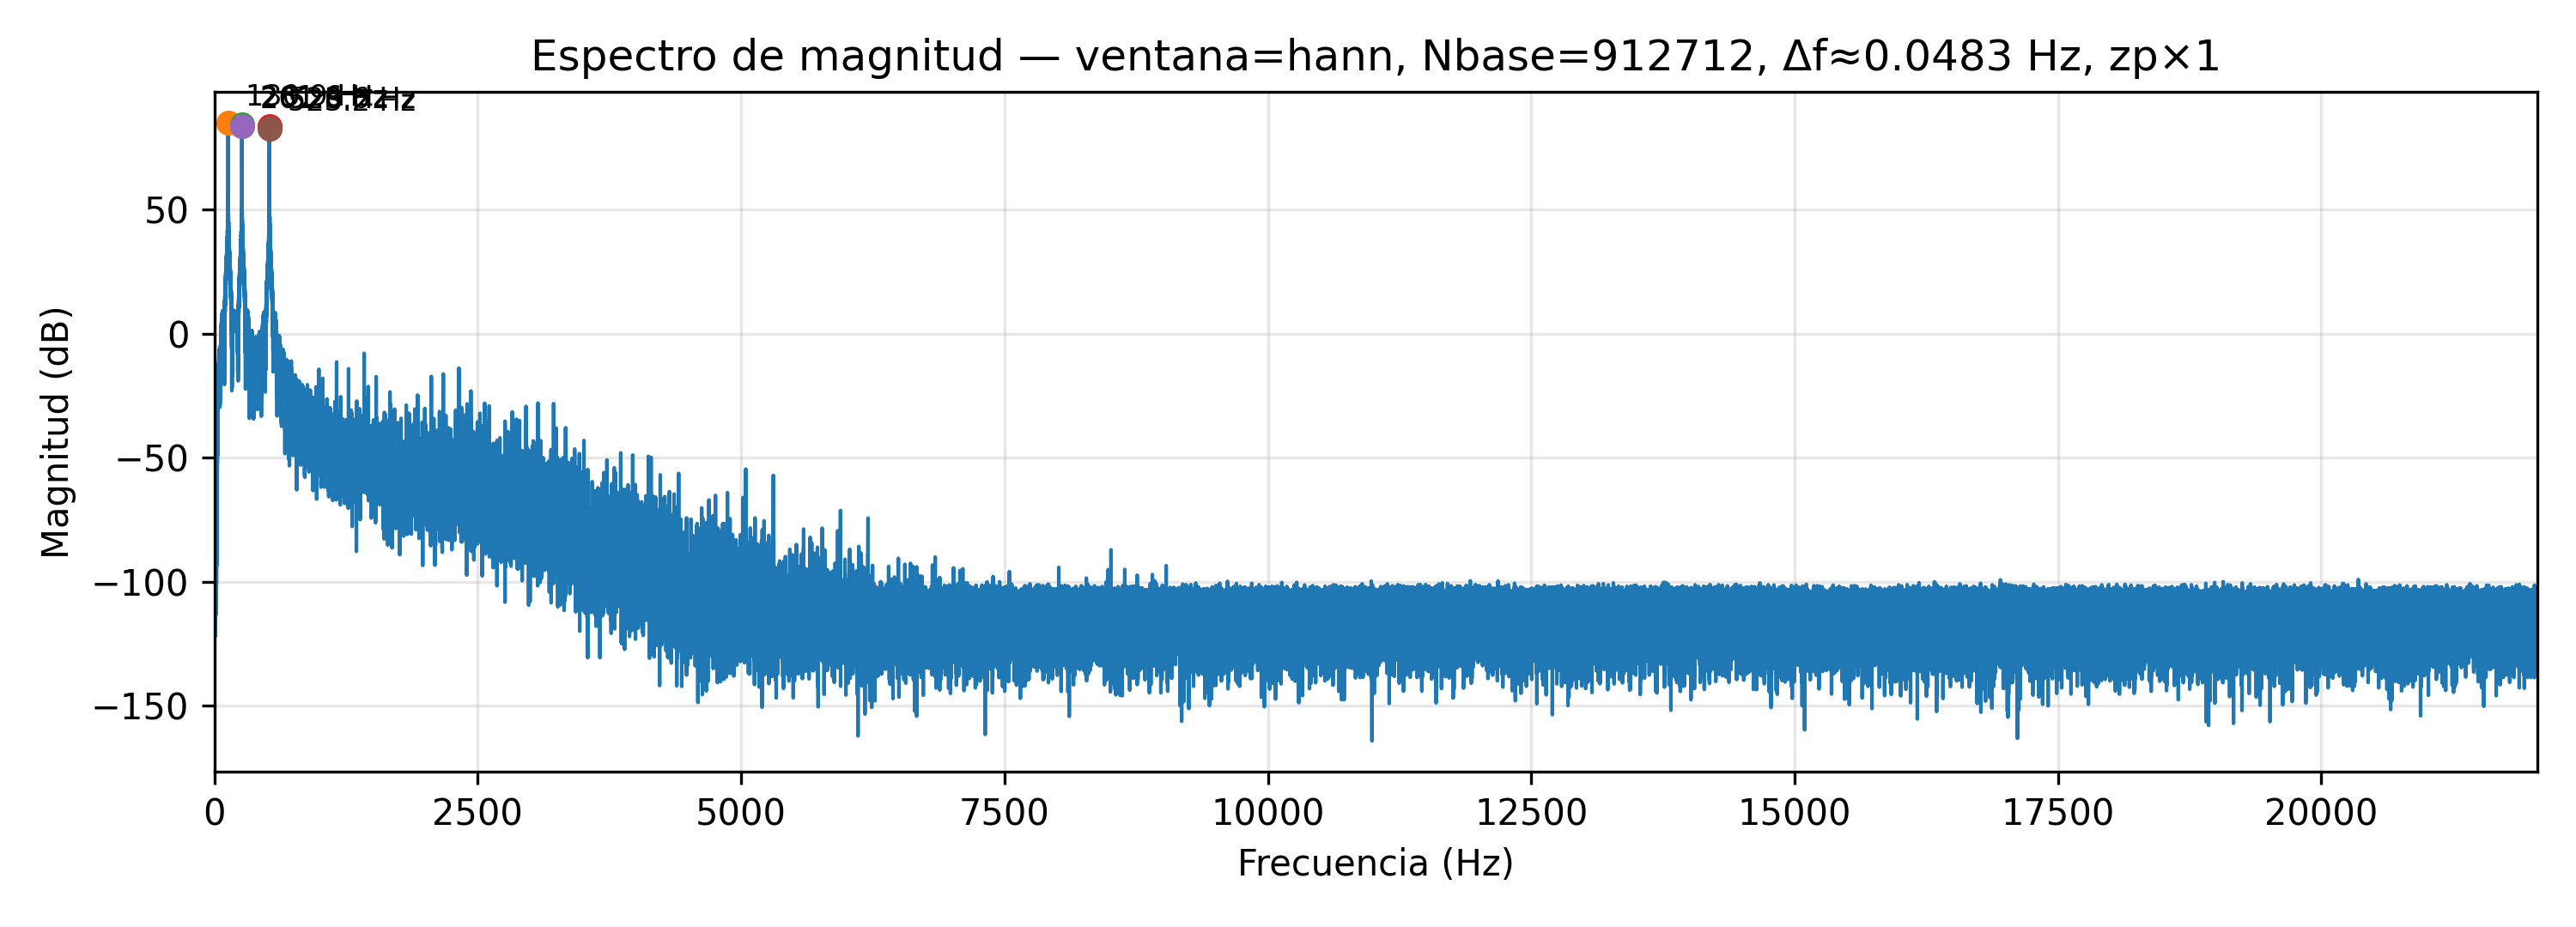
\includegraphics[width=0.98\linewidth]{Media/Figura2.png}
  \caption{Espectro de magnitud en banda completa \((0\)–\(f_s/2)\) con ventana de Hann. Se distinguen la fundamental alrededor de \(261\) Hz y octavas cercanas a \(131\) Hz y \(524\) Hz. El ventaneado reduce la fuga espectral y permite identificar los picos principales.}
  \label{fig:exp1-mag-full}
\end{figure}

La Figura~\ref{fig:exp1-mag-mid} permite distinguir el lóbulo principal de la ventana en torno a la fundamental y la estructura de lóbulos laterales. Con Hann, el primer lóbulo lateral aparece notablemente atenuado y decrece, lo que explica que el espectro fuera de la vecindad tonal permanezca bajo y estable \cite{Harris1978Windows}. El ensanchamiento del lóbulo principal observado es el comportamiento esperado de una transformada de duración finita: cuanto mayor sea \(N_{\text{base}}\), más estrecho resultará el lóbulo y mejor la separabilidad de componentes cercanas \cite{OppenheimSchaferDTSP3e}. 
% ===== Figura 3 =====
\begin{figure}[H]
  \centering
  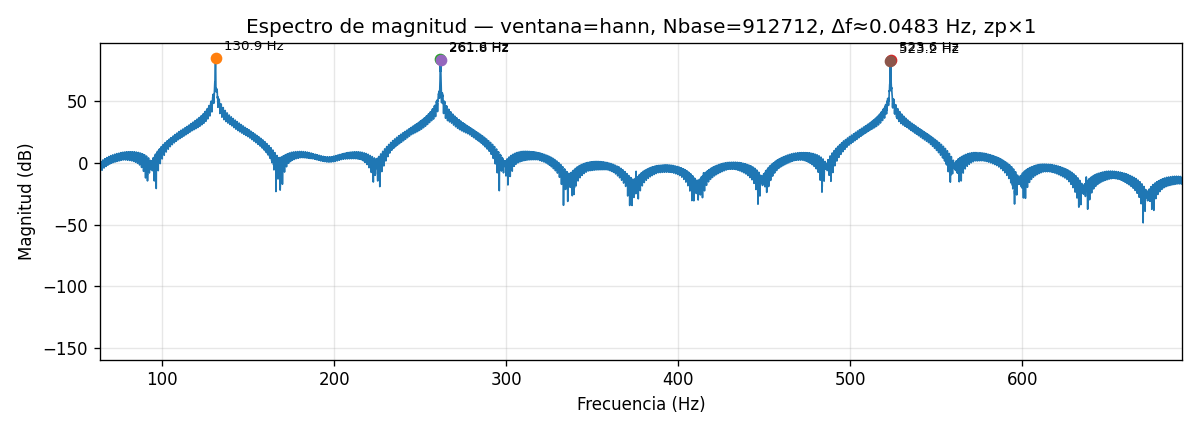
\includegraphics[width=0.98\linewidth]{Media/Figura3.png}
  \caption{Espectro de magnitud con zoom intermedio \((60\)–\(650\) Hz). Se aprecia con mayor detalle la zona tonal y los lóbulos laterales asociados al uso de la ventana de Hann.}
  \label{fig:exp1-mag-mid}
\end{figure}

En la Figura~\ref{fig:exp1-mag-zoom} se resolvió el doblete alrededor de \(261\) Hz. En la corrida mostrada, la consola reportó picos en \(f\approx 261.6\) Hz y \(f\approx 261.8\) Hz, con una separación \(\Delta f\) medida del orden de \(0.15\)–\(0.20\) Hz. Esta separación concuerda con la predicción para un intervalo de un cent alrededor de \(f_0\) (\(\Delta f_{\text{cent}} \approx f_0(2^{1/1200}-1)\)), que para \(f_0\approx 261\) Hz vale ≈\(0.15\) Hz \cite{OsgoodFTAMS2019}. La capacidad de distinguir ambas líneas está limitada por la resolución física \(\Delta f=f_s/N_{\text{base}}\); el \emph{zero padding} solo densifica la rejilla de muestreo frecuencial y mejora la lectura, pero no reduce el ancho efectivo del lóbulo ni aumenta la verdadera resolución \cite{OppenheimSchaferDTSP3e,Harris1978Windows}.

% ===== Figura 4 =====
\begin{figure}[H]
  \centering
  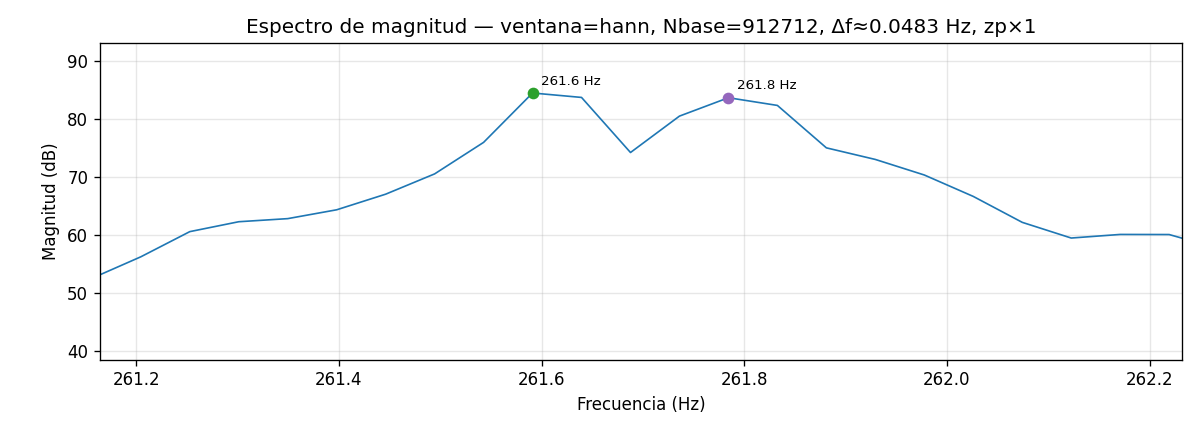
\includegraphics[width=0.98\linewidth]{Media/Figura4.png}
  \caption{Espectro de magnitud con zoom alrededor de \(261\) Hz. Se observan dos picos muy cercanos (por ejemplo, \(261.6\) Hz y \(261.8\) Hz), con separación aproximada de \(0.15\)–\(0.20\) Hz, coherente con un intervalo de un cent. El \emph{zero padding} densifica la rejilla de lectura, pero la resolución física viene dada por \(\Delta f=f_s/N_{\text{base}}\).}
  \label{fig:exp1-mag-zoom}
\end{figure}

La Figura~\ref{fig:exp1-phase} exhibe una pendiente global aproximadamente lineal de la fase con la frecuencia. Este comportamiento es característico de un desplazamiento temporal del segmento analizado: un corrimiento en tiempo introduce una rotación lineal de fase en el dominio de la frecuencia \cite{OppenheimSchaferDTSP3e,VetterliKovacevicGoyalFSP2014}. Al hacer zoom en la vecindad de las líneas alrededor de \(261\) Hz, la fase desenrollada se mantiene suave y coherente con componentes casi sinusoidales; las variaciones abruptas alejadas de las líneas se asocian a bajo nivel de señal y a los efectos del ventaneo \cite{OppenheimSchaferDTSP3e}.
% ===== Figura 5 =====
\begin{figure}[H]
  \centering
  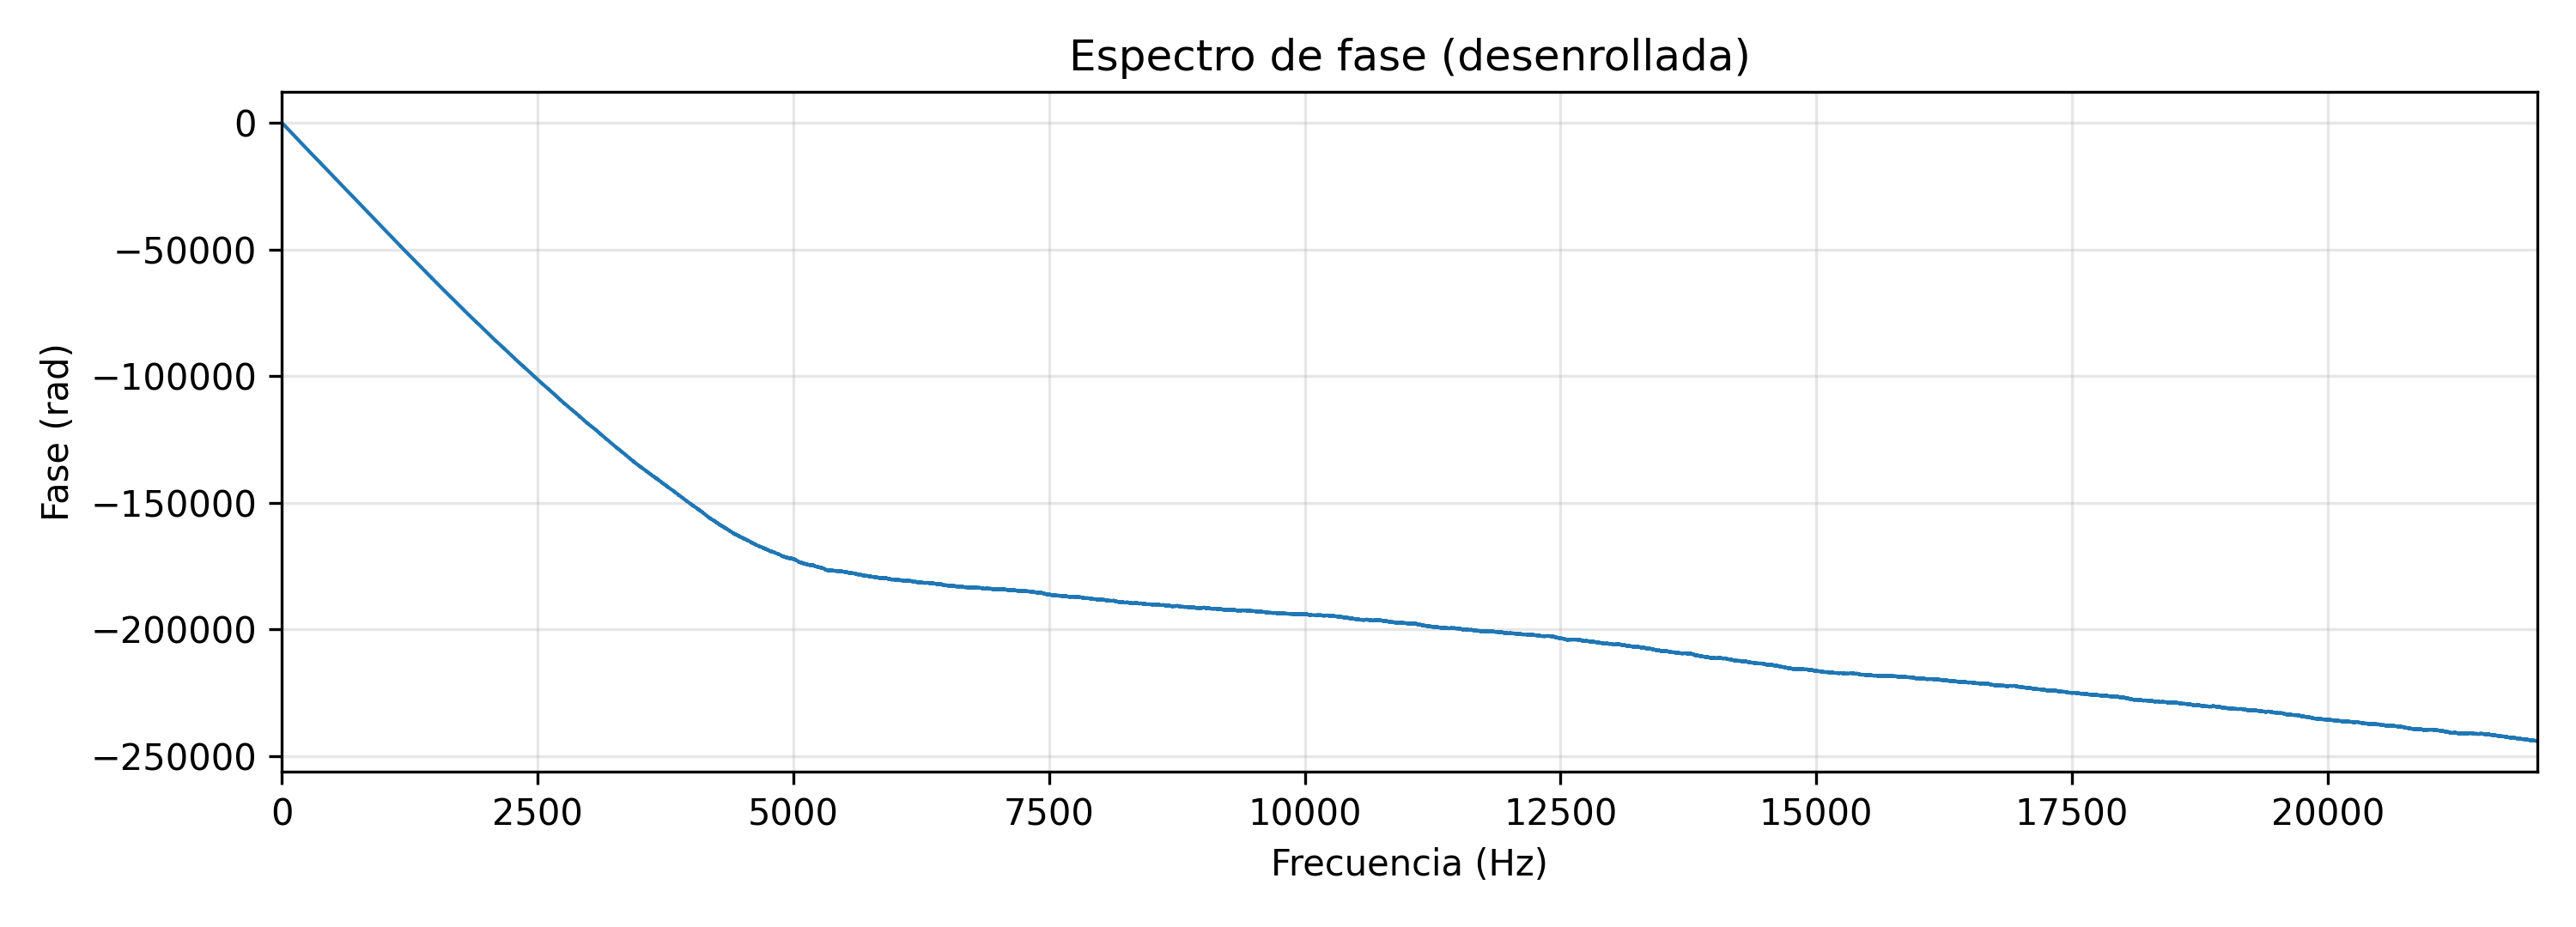
\includegraphics[width=0.98\linewidth]{Media/Figura5.png}
  \caption{Espectro de fase desenrollada. A escala ancha aparece una pendiente global asociada al origen temporal del segmento; localmente, en torno a las líneas de \(261\) Hz, la fase muestra un comportamiento suave característico de tonos casi puros.}
  \label{fig:exp1-phase}
\end{figure}  

En conjunto, los resultados confirman la relación tiempo–frecuencia esperada: la envolvente de batido en el dominio temporal y el doblete en el dominio frecuencial son dos manifestaciones del mismo fenómeno físico-matemático. La configuración empleada (Hann, \(N_{\text{base}}=912{,}712\), \(\Delta f=0.0483\) Hz) resulta suficiente para identificar el par de líneas cercanas, y la lectura es consistente con el intervalo de un cent alrededor de \(261\) Hz \cite{OppenheimSchaferDTSP3e,Harris1978Windows}.



% =========================
\section{Uso de Fourier en modulación y demodulación}
% Esta sección cubre la parte 3 (explicar a nivel de bloques cómo Fourier participa).
\subsection{Diagrama de bloques del sistema}
% - Incluir un diagrama: fuente -> modulador -> canal -> demodulador -> salida.
% - Puedes usar una figura SVG o TikZ exportada como PDF/PNG.
\begin{figure}[H]
  \centering
  \includegraphics[width=0.95\linewidth]{figs/diag_mod_demod.png} % <-- reemplaza con tu diagrama
  \caption{Diagrama de bloques del modulador-demodulador considerado.}
  \label{fig:bloques-mod-demod}
\end{figure}
\subsubsection{Señales esperadas en cada bloque}
% - Bocetos de formas de onda / espectros: banda base, portadora, bandas laterales.
% - Dónde se produce la traslación en frecuencia (mezcla), y dónde el filtrado.
\subsection{Lectura en el dominio de Fourier}
% - Explicar con palabras cómo se verían los espectros en cada etapa.
% - Vincular con filtros (PB/PBanda), sincronía y pérdidas por canal.

% =========================
\section{Bibliotecas y \emph{drivers} en microcontroladores}
% Esta sección cubre la parte 4 (bibliotecas MCU).
\subsection{Biblioteca/Driver}
% - Tabla con columnas: Bloque | MCU/Framework | Biblioteca/Driver | Comentario.
% - Ejemplos: CMSIS-DSP (ARM), ESP-DSP (ESP32), ArduinoFFT, KissFFT, ADC/DAC/I2S.

\subsubsection{Consideraciones de implementación}
% - Memoria (tamaño de buffers), tiempo real (latencias), precisión en punto fijo.
% - Consumo energético, reloj, estabilidad de osciladores.

% =========================
\section{Prototipo en PC: modulación y demodulación}
% Esta sección cubre la parte 5 (demo PC). Solo resultados e interpretación.
\subsection{Especificación del esquema de modulación}
% - Elegir uno (p.ej., AM-DSB, AM-SSB, BPSK, QPSK).
% - Parámetros: fs, fc, filtros (ancho de banda), niveles, SNR si hubo ruido simulado.
\subsubsection{Procedimiento experimental}
% - Flujo de generación: señal base -> modulador -> canal (opcional) -> demod.
% - Cómo generan figuras: script -> PNGs; lista de archivos producidos.
\subsection{Resultados en el tiempo}
% - Figuras de señal modulada y demodulada en el tiempo. Rotular ejes con unidades.
\begin{figure}[H]
  \centering
  \includegraphics[width=0.95\linewidth]{figs/mod_tiempo.png} % <-- reemplaza con tu PNG
  \caption{Señal modulada en el dominio del tiempo.}
  \label{fig:mod-tiempo}
\end{figure}
\begin{figure}[H]
  \centering
  \includegraphics[width=0.95\linewidth]{figs/demod_tiempo.png} % <-- reemplaza con tu PNG
  \caption{Señal demodulada (salida) en el dominio del tiempo.}
  \label{fig:demod-tiempo}
\end{figure}
\subsection{Resultados en frecuencia}
% - Espectros de la señal modulada y demodulada (magnitud; opcional fase).
\begin{figure}[H]
  \centering
  \includegraphics[width=0.95\linewidth]{figs/mod_frecuencia.png} % <-- reemplaza con tu PNG
  \caption{Espectro de la señal modulada.}
  \label{fig:mod-freq}
\end{figure}
\begin{figure}[H]
  \centering
  \includegraphics[width=0.95\linewidth]{figs/demod_frecuencia.png} % <-- reemplaza con tu PNG
  \caption{Espectro de la señal demodulada.}
  \label{fig:demod-freq}
\end{figure}
\subsubsection{Discusión de desempeño}
% - ¿Se recuperó correctamente la banda base? ¿Distorsión/ruido?
% - Efecto de filtros y de sincronía (portadora/fases). Limitaciones del prototipo.


    
% ====== Referencias ======
\newpage
\printbibliography

\end{document}